%%% Knitr template
%%% Ty Stanford 2015-09-01
\documentclass[11pt]{article}\usepackage[]{graphicx}\usepackage[]{color}
%% maxwidth is the original width if it is less than linewidth
%% otherwise use linewidth (to make sure the graphics do not exceed the margin)
\makeatletter
\def\maxwidth{ %
  \ifdim\Gin@nat@width>\linewidth
    \linewidth
  \else
    \Gin@nat@width
  \fi
}
\makeatother

\definecolor{fgcolor}{rgb}{0, 0, 0}
\newcommand{\hlnum}[1]{\textcolor[rgb]{0.533,0,0.133}{#1}}%
\newcommand{\hlstr}[1]{\textcolor[rgb]{0.667,0.267,0}{#1}}%
\newcommand{\hlcom}[1]{\textcolor[rgb]{1,0.533,0}{#1}}%
\newcommand{\hlopt}[1]{\textcolor[rgb]{0,0,0}{\textbf{#1}}}%
\newcommand{\hlstd}[1]{\textcolor[rgb]{0,0,0}{#1}}%
\newcommand{\hlkwa}[1]{\textcolor[rgb]{0.4,0.067,0.067}{\textbf{#1}}}%
\newcommand{\hlkwb}[1]{\textcolor[rgb]{0,0,0.4}{\textbf{#1}}}%
\newcommand{\hlkwc}[1]{\textcolor[rgb]{0,0,0.4}{#1}}%
\newcommand{\hlkwd}[1]{\textcolor[rgb]{0,0.267,0.4}{#1}}%

\usepackage{framed}
\makeatletter
\newenvironment{kframe}{%
 \def\at@end@of@kframe{}%
 \ifinner\ifhmode%
  \def\at@end@of@kframe{\end{minipage}}%
  \begin{minipage}{\columnwidth}%
 \fi\fi%
 \def\FrameCommand##1{\hskip\@totalleftmargin \hskip-\fboxsep
 \colorbox{shadecolor}{##1}\hskip-\fboxsep
     % There is no \\@totalrightmargin, so:
     \hskip-\linewidth \hskip-\@totalleftmargin \hskip\columnwidth}%
 \MakeFramed {\advance\hsize-\width
   \@totalleftmargin\z@ \linewidth\hsize
   \@setminipage}}%
 {\par\unskip\endMakeFramed%
 \at@end@of@kframe}
\makeatother

\definecolor{shadecolor}{rgb}{.97, .97, .97}
\definecolor{messagecolor}{rgb}{0, 0, 0}
\definecolor{warningcolor}{rgb}{1, 0, 1}
\definecolor{errorcolor}{rgb}{1, 0, 0}
\newenvironment{knitrout}{}{} % an empty environment to be redefined in TeX

\usepackage{alltt}

\usepackage[margin=3cm,a4paper]{geometry}
\usepackage{color}
\usepackage{amsmath}
\usepackage{amssymb}
\usepackage[utf8]{inputenc}
\usepackage[scaled=.7]{beramono}
\usepackage[T1]{fontenc}

\usepackage[hang,small,bf]{caption}
%\usepackage{subcaption}
\usepackage{natbib}
\usepackage{enumitem}
\usepackage{hyperref}
\usepackage{titlesec}
\usepackage[titletoc,toc,title]{appendix}
\usepackage[autostyle]{csquotes} 

% default font. 
% can be \sfdefault, \sfdefault or \ttdefault
%\renewcommand*{\familydefault}{\sfdefault}

%%%%%%%%%%%%%%%%%%%%% CREATE COMMANDS HERE %%%%%%%%%%%%%%%%%%%%%%

\definecolor{linkblue}{rgb}{0.192,0.494,0.675}

\newcommand{\webtext}[1]{\textcolor{linkblue}{\texttt{\footnotesize{#1}}}}
\newcommand{\byme}{\vspace{10mm}\begin{flushright}\footnotesize{Ty Stanford\\ \today}\end{flushright}\vspace{10mm}}


%%%%%%%%%%%%%%%%%%%%% PACKAGE OPTIONS %%%%%%%%%%%%%%%%%%%%%%
% caption
\setlength{\captionmargin}{30pt}
% natbib
\bibpunct{(}{)}{;}{a}{,}{,}
% enumitem
\setenumerate[1]{label=(\arabic*)}
% hyperref
\hypersetup{pdfpagemode=UseNone} % don't show bookmarks on initial view
\hypersetup{colorlinks, urlcolor={linkblue}}
% subcaption
%\captionsetup[subfigure]{labelformat=simple}
%\renewcommand\thesubfigure{(\alph{subfigure})}

\setlength{\parskip}{6pt}
\setlength{\parindent}{0pt}




%%%%%%%%%%%%%%%%%%%%% START DOC %%%%%%%%%%%%%%%%%%%%%%
\IfFileExists{upquote.sty}{\usepackage{upquote}}{}
\begin{document}

%%%%%%%%%%%%%%%%%%%%% R SETUP (NOT SHOWN) %%%%%%%%%%%%%%%%%%%%%%






\begin{center}
\Large
\textbf{Title}
\end{center}

%%%%%%%%%%%%%%%%%%%%% CHUNK OPTIONS %%%%%%%%%%%%%%%%%%%%%%
%, cache=TRUE
%, eval=FALSE
%, echo=FALSE
%, comment=NA
%, results=c('hide','hold')
%, include=TRUE
%, comment='##'
%, size='footnotesize'

%, fig.width=6
%, fig.height=6
%, out.width='0.8\\textwidth'
%, fig.cap='This is the figure caption'
%, fig.show='asis'

%%%%%%%%%%%%%%%%%%%%% FIRST CODE CHUNK %%%%%%%%%%%%%%%%%%%%%%
\begin{knitrout}\footnotesize
\definecolor{shadecolor}{rgb}{0.965, 0.965, 0.965}\color{fgcolor}\begin{kframe}
\begin{alltt}
\hlstd{n} \hlkwb{<-} \hlnum{1000}
\hlstd{x} \hlkwb{<-} \hlkwd{rnorm}\hlstd{(n)}
\hlstd{y} \hlkwb{<-} \hlkwd{rchisq}\hlstd{(n,}\hlkwc{df}\hlstd{=}\hlnum{5}\hlstd{)}
\end{alltt}
\end{kframe}
\end{knitrout}


Obtain a scatterplot of \(y\) vs \(x\). 
%%%%%%%%%%%%%%%%%%%%% SECOND CODE CHUNK %%%%%%%%%%%%%%%%%%%%%%
\begin{knitrout}\footnotesize
\definecolor{shadecolor}{rgb}{0.965, 0.965, 0.965}\color{fgcolor}\begin{kframe}
\begin{alltt}
\hlkwd{plot}\hlstd{(x, y,} \hlkwc{bty}\hlstd{=}\hlstr{"n"}\hlstd{)}
\hlstd{ch} \hlkwb{<-} \hlkwd{chull}\hlstd{(x,y)}
\hlstd{ch} \hlkwb{<-} \hlkwd{c}\hlstd{(ch,ch[}\hlnum{1}\hlstd{])}
\hlkwd{lines}\hlstd{(x[ch], y[ch],} \hlkwc{col}\hlstd{=}\hlstr{"forestgreen"}\hlstd{)}
\end{alltt}
\end{kframe}

{\centering 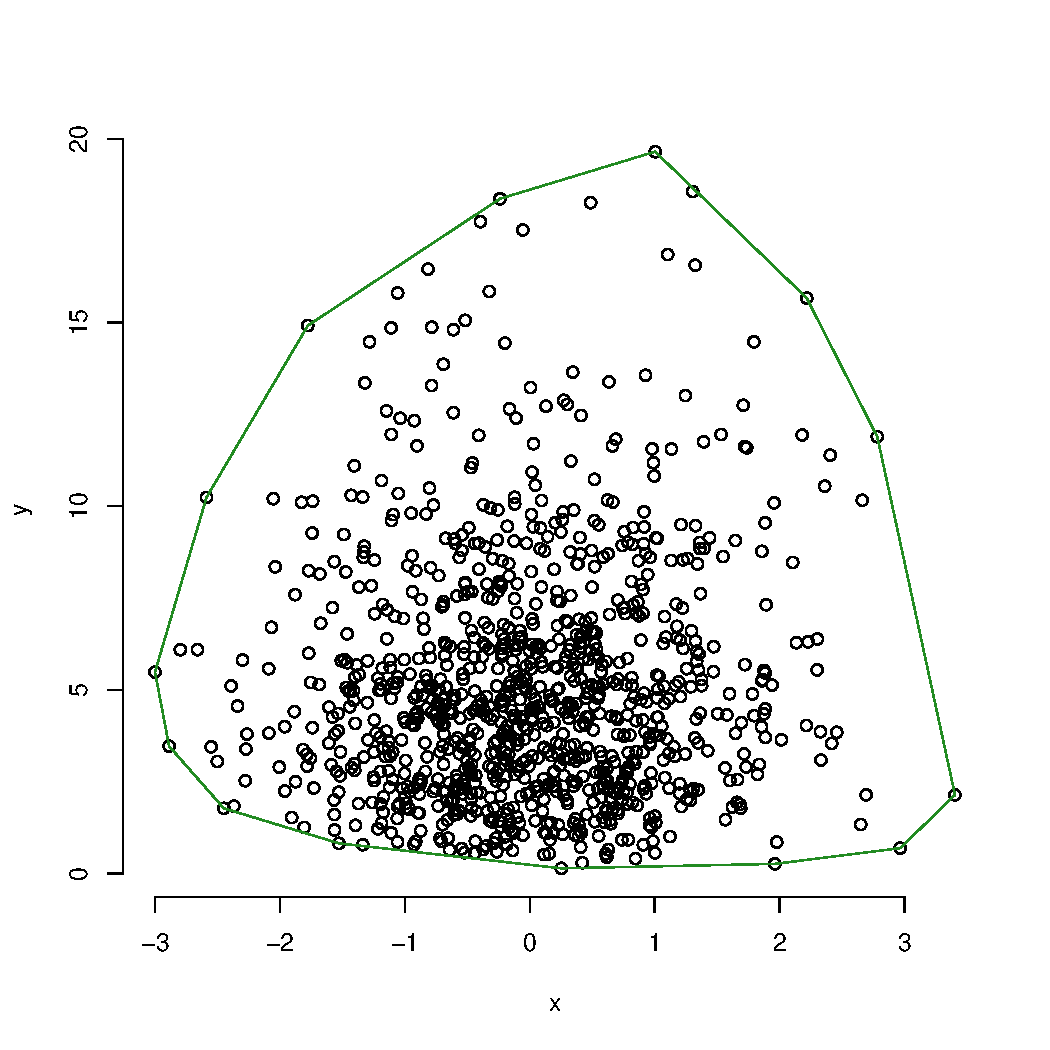
\includegraphics[width=0.6\textwidth]{fig/knitr/unnamed-chunk-1-1} 

}



\end{knitrout}


To evaluate a cached \textsf{R} object value, use the command \texttt{\textbackslash{}Sexpr\{...\}}:\\
e.g. \texttt{n}=1000.


\byme

\end{document}




%%%%%%%%%%%%%%%%%%%%% QUOTES %%%%%%%%%%%%%%%%%%%%%%

%\begin{displayquote}
%\textsl{Some quote.}
%\end{displayquote}


%%%%%%%%%%%%%%%%%%%%% FIGURE %%%%%%%%%%%%%%%%%%%%%%

%\begin{figure}[h!]
%  \centering
%    \includegraphics[width=\textwidth]{/relativefileloc/file.pdf}
%  \caption{Figure. Words.}
%\end{figure}



%%%%%%%%%%%%%%%%%%%%% SUB-FIGURES %%%%%%%%%%%%%%%%%%%%%%

%\begin{figure}[h!] 
%\centering
%	\begin{subfigure}[b]{0.49\textwidth}
%	\centering
%		\includegraphics[width=1\textwidth]{.....pdf}
%		\caption{Subcap1. } \label{sf1}
%	\end{subfigure}
%	\begin{subfigure}[b]{0.49\textwidth}
%	\centering 
%		\raisebox{0.3\height}{
%			\includegraphics[width=1\textwidth]{....pdf}
%		}
%		\caption{Subcap2. } \label{sf2}
%	\end{subfigure}
%\caption{Bottom caption.} \label{sf2}
%\end{figure}



%%%%%%%%%%%%%%%%%%%%% TABLE %%%%%%%%%%%%%%%%%%%%%%
%\begin{table}[ht]
%\centering
%\caption{Table. Words.}
%\begin{tabular}{rr}
%  \hline
%location & p.value \\ 
%  \hline
%57 & 0.0013 \\ 
%   \hline
%\end{tabular}
%\end{table}


%%%%%%%%%%%%%%%%%%%%% APPENDIX %%%%%%%%%%%%%%%%%%%%%%
%\titleformat{\section}{\large\bfseries}{\appendixname~\thesection .}{0.5em}{}
%\begin{appendices}
%\section{Some Appendix}
%The contents...
%\end{appendices}


%%%%%%%%%%%%%%%%%%%%% REFENCES %%%%%%%%%%%%%%%%%%%%%%
%\bibliographystyle{plainnat}
%\bibliography{bib} 



